\documentclass[twocolumn,oneside,a4paper]{article}
\title{極座標ステージとエクストルーダの\\同期に関する考察}
\author{青木 翔平}

\usepackage[usenames]{color} %used for font color
\usepackage{amssymb} %maths
\usepackage{amsmath} %maths
\usepackage{multirow}
\usepackage{graphicx}
\usepackage[utf8]{inputenc} %useful to type directly diacritic characters
\usepackage{algorithm}
\usepackage{algorithmic}
\usepackage{capt-of}

\renewcommand{\sectionmark}[1]{\markleft{\thesection\ #1}}

\usepackage{lastpage}
\usepackage{fancyhdr}
 \pagestyle{fancy}
%\lhead{線速度問題の解決}
\lhead{\leftmark}
\rhead{[\ \scshape\oldstylenums{\thepage}\ / %
    \scshape\oldstylenums{\pageref{LastPage}}\ ]}
 \rfoot{\copyright \hspace{0.001in} 2016. Keio University}
 
\setlength{\oddsidemargin}{0.1cm}
\setlength{\evensidemargin}{0.1cm}
\setlength{\textwidth}{50zw}

\begin{document}
\maketitle

\section{線速度について}
デカルト座標系での線速度$v$は極座標で以下のように表される.
\begin{eqnarray}
|v| &=& \sqrt{\dot{x}^2 + \dot{y}^2} \nonumber \\
  &=& \sqrt{ \left(\frac{d}{dt} r cos\theta \right) ^2 + \left(\frac{d}{dt}r sin\theta\right) ^2} \nonumber \\
  &=& \sqrt{ \dot{r}^2+ r^2 \dot{\theta}^2 } 
\end{eqnarray}	
	
いま,角速度と半径方向の速度を制御して線速度一定にすることを考える.
$v=k$(線速度一定)とすると,
\begin{eqnarray*}
  \dot{r}^2+ r^2 \dot{\theta}^2 &=& k^2 \\
  \dot{r}^2 &=&  k^2 - r^2 \dot{\theta}^2 
\end{eqnarray*}
微小区間で考えると

\begin{eqnarray}\label{eq:deltar}
	\left( \frac{\Delta r}{\Delta t}\right)^2 &=&  k^2 - r^2 \left( \frac{\Delta \theta}{\Delta t}\right)^2 \nonumber \\
|\Delta r| &=& \sqrt{(k \Delta t)^2 - (r \Delta \theta)^2}
\end{eqnarray}

いっぽう,NCコードにおいて直線移動命令G1が与えられたとき,CNCコントローラではブレゼンハムのアルゴリズム[Figure 1]にしたがって補完位置$\{x_1,x_2,...,x_n\},\{y_1,y_2,...,y_n\}$が計算される.
また,計算された$\{x_1,x_2,...,x_n\},\{y_1,y_2,...,y_n\}$は以下の関係式を用いて$\{r_1,r_2,...,r_n\},\{\theta_1,\theta_2,...,\theta_n\}$へと座標変換される. 
\begin{eqnarray*}
\left\{
  \begin{array}{ll}
r_i = \sqrt{{x_i}^2+{y_i}^2} \\	
\theta_i = tan^{-1} (y_i / x_i)
  \end{array}
  \right.
\end{eqnarray*}
すなわち,差分形式とすれば
\begin{eqnarray}\label{eq:diff}
\left\{
  \begin{array}{ll}
\Delta r = \sqrt{(\Delta x)^2+(\Delta y)^2} \\	
\Delta \theta = tan^{-1} (\Delta y / \Delta x)
  \end{array}
  \right. 
\end{eqnarray}

一般に,(\ref{eq:diff})で指定される$\Delta r, \Delta \theta$が(\ref{eq:deltar})式を満たすとは限らないため\footnote{$r$の自由度が残る.},任意の目的地の座標が指定されたときに線速度を一定にすることはできない.
%\newpage

\begin{algorithm}                  
%\captionof{algorithm}{Bresenham's algorithm}
\begin{algorithmic}                  
\label{alg1}                          
\STATE $dx \Leftarrow x1-x0$
\STATE $dy \Leftarrow y1-y0$
\STATE $D \Leftarrow 2*dy - dx$
\STATE plot(x0,y0)
\STATE $y \Leftarrow y0$
\FOR{$x$ from $x0+1$ to $x1$}
\IF{$D > 0$}
\STATE      $y \Leftarrow y+1$
\STATE      plot(x,y)
\STATE      $D \Leftarrow D + (2*dy-2*dx)$
\ELSE
\STATE      plot(x,y)
\STATE      $D \Leftarrow D + (2*dy)$
\ENDIF
\ENDFOR
\end{algorithmic}
\end{algorithm}
\captionof{figure}{Bresenham's algorithm}

\section{エクストルーダの制御について}
%\vspace{0.2in} 
ステージの変位と射出量の関係について考える.

デカルト座標系において,移動時間$\Delta t$と線速度$F$[mm/min]の関係は,以下のように表される.

\begin{eqnarray}
	\Delta t = \frac{\sqrt{(\Delta x)^2+(\Delta y)^2}}{F}\cdot 60\cdot1000
\end{eqnarray}

エクストルーダ(スクリュー)の射出量を$\Delta E_{screw}$,スクリューの回転数を$SNW$[rad/s]とおけば,以下の式が成り立つ.
\begin{eqnarray}
	\Delta E_{screw} &=& \beta \cdot (SNW) \cdot \Delta t \nonumber \\
	\therefore SNW &=& \frac{1}{\beta} \frac{\Delta E_{screw}}{\Delta t} = \beta^\prime \frac{F\cdot \Delta E_{screw}}{\sqrt{(\Delta x)^2+(\Delta y)^2}} \nonumber \\
\end{eqnarray}

前回,スライサーからの$\Delta E=E_2-E_1$を$\Delta E_{screw}$と等しいとみなして計算を行ったが,これは誤りである.なぜならば,スライサーが出力した$E$には極座標の位置による速度変化が考慮されていないからである.したがって,スライサーからのエクストルーダの値は無視する.

極座標におけるステージの線速度を$F_{polar}(t)$とすれば,微分を後退差分表示することで以下の式を得る.
\begin{eqnarray*}
F_{polar}(t_k) &=& \frac{d S}{d t}\Bigg|_{t=tk} \\
&=& \sqrt{\dot{r}^2+r^2 \dot{\theta}^2}\Big|_{t=tk} \\
&=& \sqrt{\left( \frac{r_k - r_{k-1}}{\Delta t} \right)^2 + \left(\frac{r_k+r_{k-1}}{2} \right)^2 \left( \frac{\theta_k - \theta_{k-1} }{\Delta t} \right)^2}	
\end{eqnarray*}

ステージの変位とスクリューの変位は比例するので
\begin{eqnarray}\label{eq:controller}
\int_{t_1}^{t_2} SNW(t)dt &=& \alpha \int_{t_1}^{t_2} F_{polar}(t) dt \nonumber \\
\therefore SNW\big|_{t=t_k} &=& \alpha F_{polar}(t_k)  \nonumber \\
&=& \frac{\alpha}{\Delta t} \sqrt{\left( r_k - r_{k-1} \right)^2 + \left(\frac{r_k+r_{k-1}}{2} \right)^2 \left( \theta_k - \theta_{k-1} \right)^2} \nonumber \\
&=& \frac{\alpha \cdot 60\cdot1000 \cdot \sqrt{(\Delta x)^2+(\Delta y)^2}}{F} \cdot \sqrt{\left( r_k - r_{k-1} \right)^2 + \left(\frac{r_k+r_{k-1}}{2} \right)^2  \left( \theta_k - \theta_{k-1} \right)^2} \nonumber \\
&=& \frac{\alpha^\prime}{F} \sqrt{\left( r_k - r_{k-1} \right)^2 + \left(\frac{r_k+r_{k-1}}{2} \right)^2  \left( \theta_k - \theta_{k-1} \right)^2 }  \nonumber \\
&\quad& \cdot \sqrt{ (r_k \cos\theta_k - r_{k-1} \cos\theta_{k-1})^2+(r_k \sin\theta_k - r_{k-1} \sin\theta_{k-1})^2 }
\end{eqnarray}

(\ref{eq:controller})式にしたがってスクリュー回転数を制御することで,線速度が変化する状況においてもスクリューの射出量を線速度に追従させることができる.

\clearpage

\section{予想される問題点}
\subsection{半径の近似精度} 
(\ref{eq:controller})式に表される$r_k$の計算において,$r_k$と$r_{k-1}$の平均値を用いているが,$r$が急激に増減する場合にこの部分の誤差の影響が大きくなる.一部の特殊な形状—例えば鋭利なヒトデ型—を造形する際に問題が懸念されるが,これは与えられるG-codeの半径方向の刻み($ = \Delta r$)が小さい場合,実際は問題にならないと考えられる.

\section{極座標におけるJerkについて}
前章で述べたように,極座標系において一般に線速度は一定にすることができない.$\dot{r}$と$\dot{\theta}$の振る舞いはファームウェア内で加速度を設定することで操作できるが,この際の瞬発的な加速度の増加(加加速度$\dot{a}$)を{\bf Jerk}と呼んでいる.

いま,極座標で加速度制御を行ったときに線速度のプロファイルがどのような様子を描くかに興味がある.極座標系での線速度は以下の式(\ref{eq:v})から計算できる.半径方向の速度$\dot{r}$と角速度$\dot{\theta}$を適当な台形プロファイルで仮定して数値計算した結果をFigure \ref{fig:jerk}に示す.図中の右で示される$v$が極座標系における線速度である.
\begin{eqnarray}\label{eq:v}
	|v| = \sqrt{ \dot{r}^2+ r^2 \dot{\theta}^2 } 
\end{eqnarray}

\begin{figure}[htbp]
    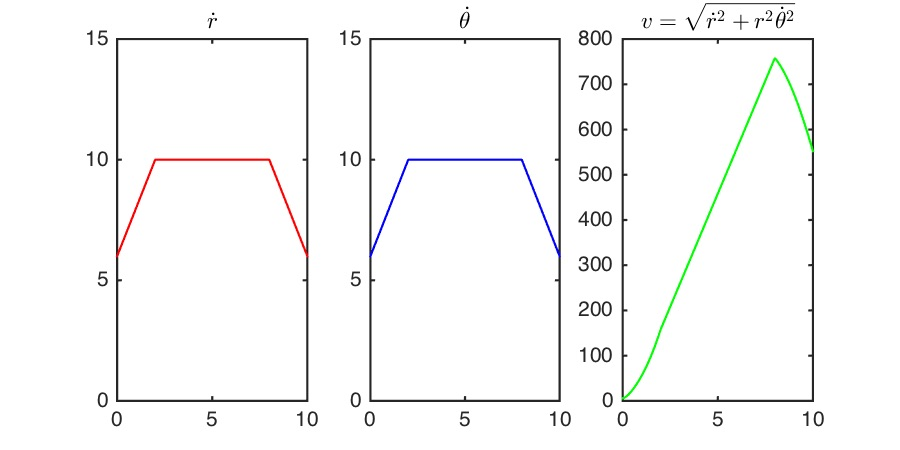
\includegraphics[bb=0 0 432 216,width=1\columnwidth]{accel2.pdf}
    \caption{Velocity profile}
    \label{fig:jerk}
\end{figure}

Figure \ref{fig:jerk}から,$\dot{r}$と$\dot{\theta}$を台形型の速度プロファイルで制御したとしても,線速度は台形型とならないことがわかる.これはデカルト座標系との違いである.

補足として,Jerkをゼロとした時の計算結果をFigure \ref{fig:jerk}に示す.
\begin{figure}[t]
    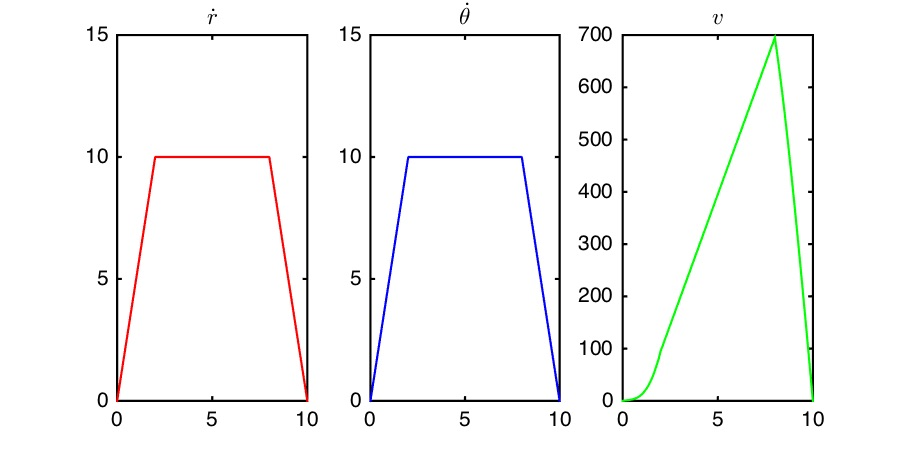
\includegraphics[bb=0 0 432 216,width=1\columnwidth]{accel.pdf}
    \caption{Velocity profile (non jerk)}
    \label{fig:jerk_zero}
\end{figure}
最高到達速度が少し低くなっているのと,終端速度がゼロになることがわかる.

\begin{thebibliography}{99}
  \bibitem{joshiki} 伊理正夫,藤野和建,『数値計算の常識』,共立出版 (1985)
\end{thebibliography}

%またこのとき,極座標系での移動変位はFigure \ref{fig:displacement}に示すように遷移している.
%\begin{figure}[htbp]
%    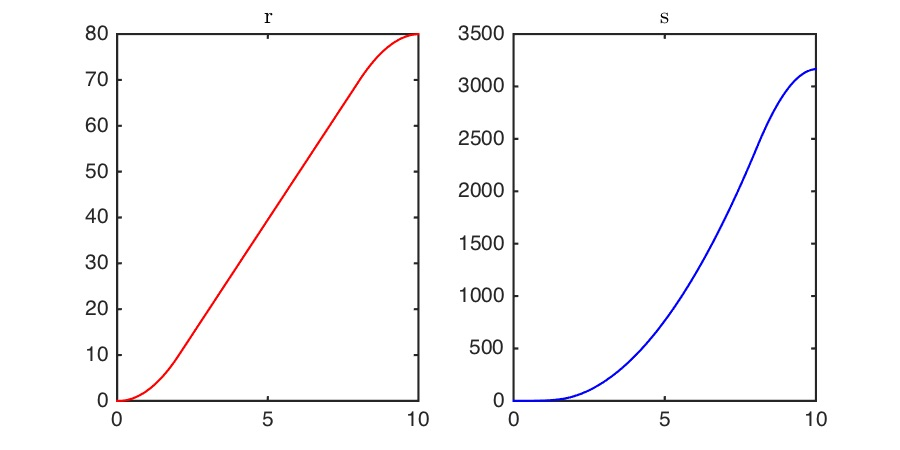
\includegraphics[bb=0 0 432 216,width=9cm]{displacement.pdf}
%    \caption{Travel distance}
%    \label{fig:displacement}
%\end{figure}

%$\dot{v} = 0$より,
%\begin{eqnarray}
%    
%	\frac{d}{dt} \left(\sqrt{ \dot{r}^2+ r^2 \dot{\theta}^2 } \right) &=& 0 \nonumber \\
%\frac{1}{2\sqrt{ \dot{r}^2+ r^2 \theta^2 }} \cdot \frac{d}{dt}\left( \dot{r}^2+r^2 \dot{\theta}^2 \right) &=& 0 \nonumber \\ 
%\frac{2\dot{r}\ddot{r} + 2r\dot{r}\dot{\theta}^2 + 2r^2\dot{\theta}\ddot{\theta}}{2\sqrt{ \dot{r}^2+ r^2 \theta^2 }} &=& 0 \nonumber \\
%\dot{r}\ddot{r} + r\dot{r}\dot{\theta}^2 + r^2\dot{\theta}\ddot{\theta} &=& 0  
%\end{eqnarray}
%	
%以上を満たすように$r$と$\theta$を制御する必要がある.
%	
%(2)式をさらに計算する.
%$\dot{\theta}=\omega$とおいて,
%\begin{eqnarray}
%  \dot{r}\ddot{r}+r\omega(\dot{r}\omega+r\dot{\omega})&=&0 \nonumber \\
%  \dot{r}\ddot{r} &=& -r\omega\frac{d}{dt}(r\omega) 
%\end{eqnarray}
%$\dot{r}=x, r\omega=y$とおくと,
%\begin{eqnarray}
%  x\frac{dx}{dt} &=& -y\frac{dy}{dt} \nonumber \\
%  xdx + ydy &=& 0	
%\end{eqnarray}
%
%(4)式は完全微分形の微分方程式である.(4)を解くと,
%\begin{eqnarray}
%  x^2+y^2 &=& C  \nonumber \\
%  \dot{r}^2 + (r\omega)^2 &=& C \nonumber \\
%  \dot{r}^2 &=& -(r\omega)^2 + C 	
%\end{eqnarray}
%初期条件$t=0, r=a, \dot{r}=0, \omega=\omega_0$とすると,
%\begin{eqnarray*}
%  C=a^2\omega_0^2	
%\end{eqnarray*}
%したがって,
%\begin{eqnarray}
%  \dot{r}^2 &=& a^2 \omega_0^2 - r^2 \omega^2 \nonumber \\
%  \dot{r}^2 - a^2 \omega_0^2 &=& r^2 \omega^2 \nonumber \\
%  \omega^2 &=& \frac{1}{r^2} \left\{ \dot{r}^2 - a^2 {\omega_0}^2  \right\} \nonumber \\
%  \omega &=& \frac{1}{r} \sqrt{ \dot{r}^2 - a^2 {\omega_0}^2 }  
%\end{eqnarray}



\end{document}